\documentclass[12pt,a4paper]{article}
\usepackage[utf8]{inputenc}
\usepackage{amsmath}
\usepackage{amsfonts}
\usepackage{amssymb}
\usepackage{graphicx}
\usepackage{geometry}
\usepackage{fancyhdr}
\usepackage{xcolor}
\usepackage{tcolorbox}
\usepackage{hyperref}
\usepackage{tikz}
\usetikzlibrary{shapes,arrows,positioning}

\geometry{margin=1in}
\pagestyle{fancy}
\fancyhf{}
\rhead{BlocTime Protocol}
\lhead{Whitepaper}
\cfoot{\thepage}

\definecolor{primaryblue}{RGB}{0,51,102}
\definecolor{accentgold}{RGB}{218,165,32}
\definecolor{treasurygreen}{RGB}{34,139,34}

\title{\Huge\textbf{\textcolor{primaryblue}{BlocTime Protocol}}\\[0.5cm]
\Large\textit{Sustainable Revenue-Sharing Tokenomics}\\[0.3cm]
\large\textcolor{accentgold}{Whitepaper}\\[0.2cm]
\normalsize\textit{Where Mathematics Meets Economics}}
\author{BlocTime Research Team}
\date{\today}

\begin{document}

\maketitle
\thispagestyle{empty}

\begin{center}
\vspace{2cm}
\textit{"Everything should be made as simple as possible, but not simpler."}\\
--- Albert Einstein
\vspace{1cm}

\textit{"Simplicity is the ultimate sophistication."}\\
--- Leonardo da Vinci
\end{center}

\newpage
\tableofcontents
\newpage

\section{Executive Summary}

BlocTime Protocol introduces a revolutionary approach to decentralized finance by creating a \textbf{self-sustaining economic ecosystem} where token holders earn passive income from real marketplace revenue, not from inflationary token emissions.

\subsection{The Problem}

Traditional staking protocols suffer from fundamental flaws:

\begin{itemize}
    \item \textbf{Inflationary Rewards}: New tokens dilute existing holders
    \item \textbf{Unsustainable APYs}: High yields collapse as supply increases
    \item \textbf{Misaligned Incentives}: Stakers don't benefit from ecosystem growth
    \item \textbf{Manual Treasury Management}: Requires centralized intervention
\end{itemize}

\subsection{The Solution}

BlocTime creates a unified staking and marketplace system where:

\begin{tcolorbox}[colback=primaryblue!5,colframe=primaryblue,title=Core Innovation]
\textbf{100\% of marketplace fees automatically flow to stakers}, proportional to their commitment, creating sustainable passive income from real economic activity.
\end{tcolorbox}

\subsection{Key Features}

\begin{enumerate}
    \item \textbf{Time-Locked Staking}: Earn up to 3x multiplier for longer commitments
    \item \textbf{Automatic Revenue Sharing}: No manual claims or distributions
    \item \textbf{Fractional Marketplace}: Rent computing power, AI models, digital assets by the block
    \item \textbf{Secondary Market}: Resell unused rental time
    \item \textbf{Zero Inflation}: Rewards from real revenue, not token printing
\end{enumerate}

\section{The BlocTime Ecosystem}

\subsection{System Architecture}

The protocol consists of three interconnected components:

\begin{center}
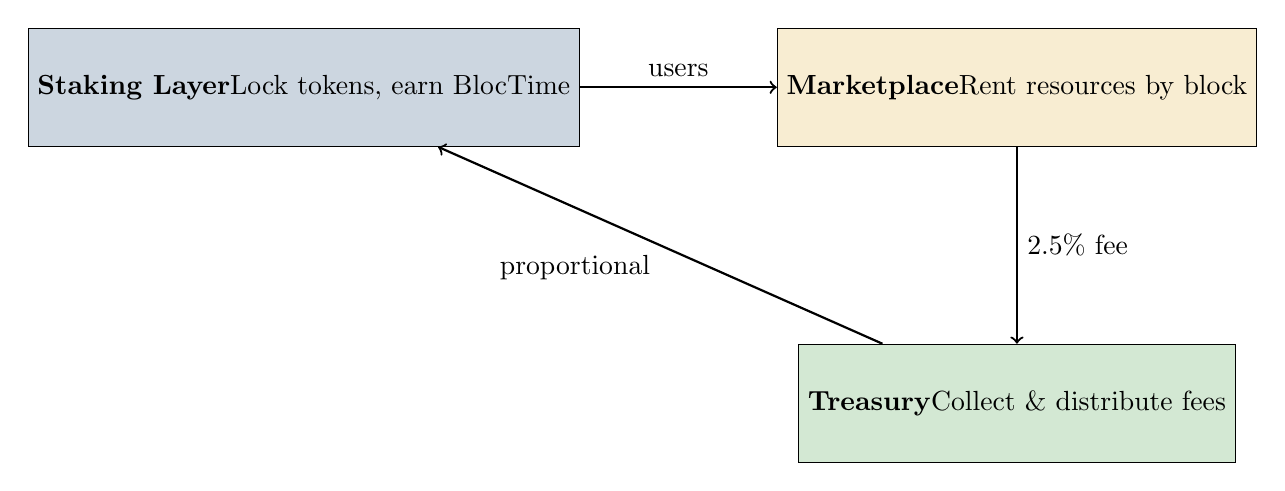
\begin{tikzpicture}[node distance=2.5cm, auto]
  \node[draw, rectangle, fill=primaryblue!20, minimum width=3cm, minimum height=1.5cm] (staking) {\textbf{Staking Layer}\\Lock tokens, earn BlocTime};
  \node[draw, rectangle, fill=accentgold!20, minimum width=3cm, minimum height=1.5cm, right=of staking] (marketplace) {\textbf{Marketplace}\\Rent resources by block};
  \node[draw, rectangle, fill=treasurygreen!20, minimum width=3cm, minimum height=1.5cm, below=of marketplace] (treasury) {\textbf{Treasury}\\Collect \& distribute fees};
  
  \draw[->, thick] (marketplace) -- node {2.5\% fee} (treasury);
  \draw[->, thick] (treasury) -- node {proportional} (staking);
  \draw[->, thick] (staking) -- node {users} (marketplace);
\end{tikzpicture}
\end{center}

\subsection{How It Works}

\subsubsection{For Token Holders (Stakers)}

\begin{enumerate}
    \item \textbf{Lock Tokens}: Choose lock duration (0 to 100,000+ blocks)
    \item \textbf{Receive BlocTime}: Get 1x to 3x multiplier based on commitment
    \item \textbf{Earn Automatically}: Receive share of ALL marketplace fees
    \item \textbf{Claim Anytime}: Withdraw rewards without unstaking
    \item \textbf{Unlock Later}: Retrieve original tokens after lock period
\end{enumerate}

\subsubsection{For Marketplace Users}

\begin{enumerate}
    \item \textbf{Browse Resources}: Computing power, AI models, digital assets
    \item \textbf{Rent by Block}: Pay only for what you need
    \item \textbf{Use Resources}: Access during rental period
    \item \textbf{Resell Unused Time}: List fractional blocks on secondary market
\end{enumerate}

\section{Mathematical Framework}

\subsection{BlocTime Token Minting}

When staking amount $S$ for duration $D$ blocks:

\begin{tcolorbox}[colback=primaryblue!5,colframe=primaryblue,title=Minting Formula]
\begin{equation}
\boxed{B_{\text{earned}} = S \times M(D)}
\end{equation}

Where $M(D)$ is the multiplier function:
\begin{itemize}
    \item $M(0) = 1.0x$ (instant unlock)
    \item $M(10,000) = 1.5x$ (~1.5 days)
    \item $M(50,000) = 2.0x$ (~1 week)
    \item $M(100,000) = 3.0x$ (~2 weeks)
\end{itemize}
\end{tcolorbox}

\subsection{Revenue Distribution}

Your share of marketplace revenue:

\begin{tcolorbox}[colback=treasurygreen!5,colframe=treasurygreen,title=Reward Formula]
\begin{equation}
\boxed{R_{\text{user}} = \frac{B_{\text{user}}}{B_{\text{total}}} \times T \times \delta}
\end{equation}

Where:
\begin{itemize}
    \item $B_{\text{user}}$ = Your BlocTime balance
    \item $B_{\text{total}}$ = Total BlocTime in circulation
    \item $T$ = Treasury balance
    \item $\delta$ = Distribution rate (50\% default)
\end{itemize}
\end{tcolorbox}

\subsection{Marketplace Fee Structure}

Every transaction generates revenue:

\begin{align}
\text{Total Cost} &= \text{Blocks} \times \text{Price per Block} \\
\text{Treasury Fee} &= \text{Total Cost} \times 2.5\% \\
\text{Owner Payment} &= \text{Total Cost} \times 97.5\%
\end{align}

\section{Economic Model}

\subsection{The Virtuous Cycle}

\begin{center}
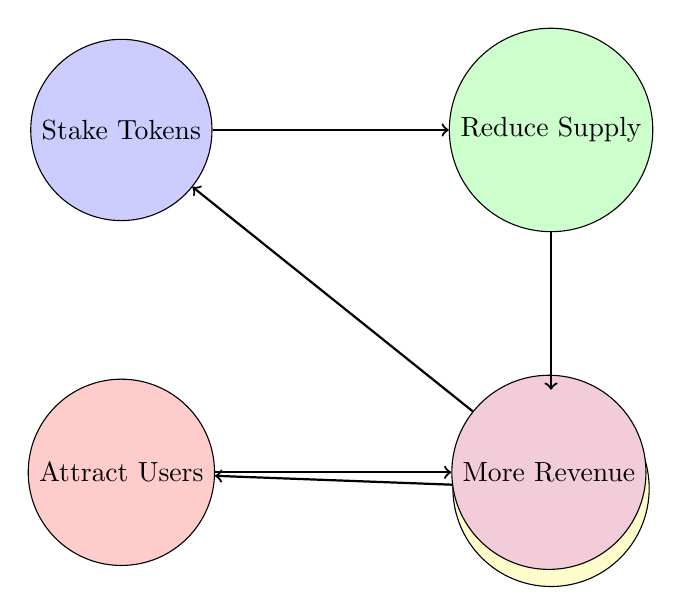
\begin{tikzpicture}[node distance=2cm, auto]
  \node[draw, circle, fill=blue!20] (stake) {Stake Tokens};
  \node[draw, circle, fill=green!20, right=of stake, xshift=1cm] (reduce) {Reduce Supply};
  \node[draw, circle, fill=yellow!20, below=of reduce] (value) {Increase Value};
  \node[draw, circle, fill=red!20, below=of stake] (users) {Attract Users};
  \node[draw, circle, fill=purple!20, right=of users, xshift=1cm] (revenue) {More Revenue};
  
  \draw[->, thick] (stake) -- (reduce);
  \draw[->, thick] (reduce) -- (value);
  \draw[->, thick] (value) -- (users);
  \draw[->, thick] (users) -- (revenue);
  \draw[->, thick] (revenue) -- (stake);
\end{tikzpicture}
\end{center}

\subsection{Real-World Example}

\textbf{Scenario}: You stake 1,000 tokens for 50,000 blocks (1 week)

\begin{enumerate}
    \item \textbf{BlocTime Earned}: $1,000 \times 2.0 = 2,000$ BlocTime
    \item \textbf{Total BlocTime}: 100,000 (example)
    \item \textbf{Your Share}: $2,000 / 100,000 = 2\%$
    \item \textbf{Monthly Marketplace Fees}: \$10,000
    \item \textbf{Distribution Pool}: $\$10,000 \times 50\% = \$5,000$
    \item \textbf{Your Monthly Reward}: $\$5,000 \times 2\% = \$100$
\end{enumerate}

\textbf{Annual Return}: $\$100 \times 12 = \$1,200$ on \$1,000 stake = \textbf{120\% APY}

\textit{Note: Returns scale with marketplace growth, not fixed APY}

\section{Marketplace Features}

\subsection{What Can Be Rented?}

\begin{itemize}
    \item \textbf{Computing Resources}: GPU clusters, CPU nodes, storage
    \item \textbf{AI Models}: Language models, image generators, data processors
    \item \textbf{Digital Assets}: Software licenses, API access, premium content
    \item \textbf{Custom Modules}: Any tokenizable resource
\end{itemize}

\subsection{Fractional Rentals}

Rent 1,000 blocks but only need 600? \textbf{Sell the remaining 400}:

\begin{tcolorbox}[colback=accentgold!5,colframe=accentgold,title=Secondary Market]
\begin{itemize}
    \item List unused block ranges for sale
    \item Set your own price
    \item Buyers get instant access
    \item Sellers recover costs
    \item Treasury earns 2.5\% on resales too
\end{itemize}
\end{tcolorbox}

\section{Security \& Trust}

\subsection{Smart Contract Security}

\begin{enumerate}
    \item \textbf{OpenZeppelin Standards}: Battle-tested contract libraries
    \item \textbf{ReentrancyGuard}: Protection against reentrancy attacks
    \item \textbf{SafeERC20}: Safe token transfer operations
    \item \textbf{Overflow Protection}: Solidity 0.8+ built-in checks
    \item \textbf{Access Control}: Owner-only administrative functions
\end{enumerate}

\subsection{Economic Security}

\begin{itemize}
    \item \textbf{No Flash Loan Exploits}: Lock periods prevent instant unstaking
    \item \textbf{Sybil Resistance}: Rewards require real token commitment
    \item \textbf{Fair Distribution}: Proportional rewards regardless of claim order
    \item \textbf{No Admin Keys}: Core functions are immutable
\end{itemize}

\section{Comparison with Alternatives}

\begin{center}
\begin{tabular}{|l|c|c|}
\hline
\textbf{Feature} & \textbf{Traditional Staking} & \textbf{BlocTime} \\
\hline
Reward Source & Token Inflation & Real Revenue \\
Sustainability & Decreasing APY & Growth-Based \\
Ecosystem Alignment & No & Yes \\
Manual Management & Required & Automatic \\
Value Dilution & Yes & No \\
Marketplace Integration & No & Yes \\
\hline
\end{tabular}
\end{center}

\section{Roadmap}

\subsection{Phase 1: Foundation (Complete)}
\begin{itemize}
    \item ✅ Core smart contracts deployed
    \item ✅ Staking with multipliers
    \item ✅ Basic marketplace
    \item ✅ Treasury integration
\end{itemize}

\subsection{Phase 2: Enhancement (Current)}
\begin{itemize}
    \item ✅ Fractional rentals
    \item ✅ Secondary market
    \item 🔄 Advanced analytics
    \item 🔄 Mobile interface
\end{itemize}

\subsection{Phase 3: Expansion (Planned)}
\begin{itemize}
    \item 📋 Governance system
    \item 📋 Multi-chain deployment
    \item 📋 NFT integration
    \item 📋 Cross-chain bridges
\end{itemize}

\section{Team \& Community}

\subsection{Core Values}

\begin{itemize}
    \item \textbf{Transparency}: All code is open-source
    \item \textbf{Simplicity}: Elegant solutions over complexity
    \item \textbf{Sustainability}: Long-term thinking
    \item \textbf{Community}: Decentralized governance
\end{itemize}

\section{Getting Started}

\subsection{For Stakers}

\begin{enumerate}
    \item Acquire protocol tokens
    \item Connect wallet to BlocTime dApp
    \item Choose lock duration (longer = higher multiplier)
    \item Approve and stake tokens
    \item Receive BlocTime tokens
    \item Watch rewards accumulate
    \item Claim rewards anytime
    \item Unstake after lock period
\end{enumerate}

\subsection{For Marketplace Users}

\begin{enumerate}
    \item Browse available resources
    \item Select rental duration (in blocks)
    \item Pay for rental
    \item Access resource during rental period
    \item (Optional) List unused blocks for resale
\end{enumerate}

\section{Conclusion}

BlocTime Protocol represents a paradigm shift in decentralized finance:

\begin{tcolorbox}[colback=primaryblue!5,colframe=primaryblue,title=The BlocTime Promise]
\begin{itemize}
    \item \textbf{Sustainable}: Revenue from real economic activity
    \item \textbf{Automatic}: No manual intervention required
    \item \textbf{Fair}: Proportional rewards for all participants
    \item \textbf{Aligned}: Everyone benefits from ecosystem growth
    \item \textbf{Simple}: Elegant mathematics, robust engineering
\end{itemize}
\end{tcolorbox}

\vspace{1cm}

\begin{center}
\textcolor{primaryblue}{\textbf{\Large Join the BlocTime Revolution}}\\
\vspace{0.5cm}
\textcolor{accentgold}{\textit{Where Your Commitment Earns Real Rewards}}\\
\vspace{0.5cm}
\textcolor{treasurygreen}{\textit{Built with 💎 by the BlocTime Team}}
\end{center}

\appendix

\section{Technical Specifications}

\subsection{Contract Addresses}

\textit{See technical documentation for deployment addresses}

\subsection{Gas Costs}

\begin{center}
\begin{tabular}{|l|r|}
\hline
\textbf{Operation} & \textbf{Estimated Gas} \\
\hline
Stake & ~150,000 \\
Unstake & ~100,000 \\
Claim Rewards & ~80,000 \\
Rent Module & ~200,000 \\
List Fractional & ~120,000 \\
Buy Listing & ~180,000 \\
\hline
\end{tabular}
\end{center}

\section{Legal Disclaimer}

This whitepaper is for informational purposes only. BlocTime Protocol does not constitute financial advice. Cryptocurrency investments carry risk. Please conduct your own research and consult with financial advisors before participating.

\section{Contact \& Resources}

\begin{itemize}
    \item \textbf{Website}: https://bloctime.io
    \item \textbf{GitHub}: https://github.com/bloctime
    \item \textbf{Documentation}: See technical docs
    \item \textbf{Community}: Discord/Telegram links
\end{itemize}

\end{document}